% Options for packages loaded elsewhere
\PassOptionsToPackage{unicode}{hyperref}
\PassOptionsToPackage{hyphens}{url}
%
\documentclass[
  ignorenonframetext,
]{beamer}
\usepackage{pgfpages}
\setbeamertemplate{caption}[numbered]
\setbeamertemplate{caption label separator}{: }
\setbeamercolor{caption name}{fg=normal text.fg}
\beamertemplatenavigationsymbolsempty
% Prevent slide breaks in the middle of a paragraph
\widowpenalties 1 10000
\raggedbottom
\setbeamertemplate{part page}{
  \centering
  \begin{beamercolorbox}[sep=16pt,center]{part title}
    \usebeamerfont{part title}\insertpart\par
  \end{beamercolorbox}
}
\setbeamertemplate{section page}{
  \centering
  \begin{beamercolorbox}[sep=12pt,center]{part title}
    \usebeamerfont{section title}\insertsection\par
  \end{beamercolorbox}
}
\setbeamertemplate{subsection page}{
  \centering
  \begin{beamercolorbox}[sep=8pt,center]{part title}
    \usebeamerfont{subsection title}\insertsubsection\par
  \end{beamercolorbox}
}
\AtBeginPart{
  \frame{\partpage}
}
\AtBeginSection{
  \ifbibliography
  \else
    \frame{\sectionpage}
  \fi
}
\AtBeginSubsection{
  \frame{\subsectionpage}
}
\usepackage{lmodern}
\usepackage{amssymb,amsmath}
\usepackage{ifxetex,ifluatex}
\ifnum 0\ifxetex 1\fi\ifluatex 1\fi=0 % if pdftex
  \usepackage[T1]{fontenc}
  \usepackage[utf8]{inputenc}
  \usepackage{textcomp} % provide euro and other symbols
\else % if luatex or xetex
  \usepackage{unicode-math}
  \defaultfontfeatures{Scale=MatchLowercase}
  \defaultfontfeatures[\rmfamily]{Ligatures=TeX,Scale=1}
\fi
% Use upquote if available, for straight quotes in verbatim environments
\IfFileExists{upquote.sty}{\usepackage{upquote}}{}
\IfFileExists{microtype.sty}{% use microtype if available
  \usepackage[]{microtype}
  \UseMicrotypeSet[protrusion]{basicmath} % disable protrusion for tt fonts
}{}
\makeatletter
\@ifundefined{KOMAClassName}{% if non-KOMA class
  \IfFileExists{parskip.sty}{%
    \usepackage{parskip}
  }{% else
    \setlength{\parindent}{0pt}
    \setlength{\parskip}{6pt plus 2pt minus 1pt}}
}{% if KOMA class
  \KOMAoptions{parskip=half}}
\makeatother
\usepackage{xcolor}
\IfFileExists{xurl.sty}{\usepackage{xurl}}{} % add URL line breaks if available
\IfFileExists{bookmark.sty}{\usepackage{bookmark}}{\usepackage{hyperref}}
\hypersetup{
  pdftitle={Inferens i mixed models i R - hinsides det sædvanlige likelihood ratio test},
  hidelinks,
  pdfcreator={LaTeX via pandoc}}
\urlstyle{same} % disable monospaced font for URLs
\newif\ifbibliography
\usepackage{color}
\usepackage{fancyvrb}
\newcommand{\VerbBar}{|}
\newcommand{\VERB}{\Verb[commandchars=\\\{\}]}
\DefineVerbatimEnvironment{Highlighting}{Verbatim}{commandchars=\\\{\}}
% Add ',fontsize=\small' for more characters per line
\usepackage{framed}
\definecolor{shadecolor}{RGB}{248,248,248}
\newenvironment{Shaded}{\begin{snugshade}}{\end{snugshade}}
\newcommand{\AlertTok}[1]{\textcolor[rgb]{0.94,0.16,0.16}{#1}}
\newcommand{\AnnotationTok}[1]{\textcolor[rgb]{0.56,0.35,0.01}{\textbf{\textit{#1}}}}
\newcommand{\AttributeTok}[1]{\textcolor[rgb]{0.77,0.63,0.00}{#1}}
\newcommand{\BaseNTok}[1]{\textcolor[rgb]{0.00,0.00,0.81}{#1}}
\newcommand{\BuiltInTok}[1]{#1}
\newcommand{\CharTok}[1]{\textcolor[rgb]{0.31,0.60,0.02}{#1}}
\newcommand{\CommentTok}[1]{\textcolor[rgb]{0.56,0.35,0.01}{\textit{#1}}}
\newcommand{\CommentVarTok}[1]{\textcolor[rgb]{0.56,0.35,0.01}{\textbf{\textit{#1}}}}
\newcommand{\ConstantTok}[1]{\textcolor[rgb]{0.00,0.00,0.00}{#1}}
\newcommand{\ControlFlowTok}[1]{\textcolor[rgb]{0.13,0.29,0.53}{\textbf{#1}}}
\newcommand{\DataTypeTok}[1]{\textcolor[rgb]{0.13,0.29,0.53}{#1}}
\newcommand{\DecValTok}[1]{\textcolor[rgb]{0.00,0.00,0.81}{#1}}
\newcommand{\DocumentationTok}[1]{\textcolor[rgb]{0.56,0.35,0.01}{\textbf{\textit{#1}}}}
\newcommand{\ErrorTok}[1]{\textcolor[rgb]{0.64,0.00,0.00}{\textbf{#1}}}
\newcommand{\ExtensionTok}[1]{#1}
\newcommand{\FloatTok}[1]{\textcolor[rgb]{0.00,0.00,0.81}{#1}}
\newcommand{\FunctionTok}[1]{\textcolor[rgb]{0.00,0.00,0.00}{#1}}
\newcommand{\ImportTok}[1]{#1}
\newcommand{\InformationTok}[1]{\textcolor[rgb]{0.56,0.35,0.01}{\textbf{\textit{#1}}}}
\newcommand{\KeywordTok}[1]{\textcolor[rgb]{0.13,0.29,0.53}{\textbf{#1}}}
\newcommand{\NormalTok}[1]{#1}
\newcommand{\OperatorTok}[1]{\textcolor[rgb]{0.81,0.36,0.00}{\textbf{#1}}}
\newcommand{\OtherTok}[1]{\textcolor[rgb]{0.56,0.35,0.01}{#1}}
\newcommand{\PreprocessorTok}[1]{\textcolor[rgb]{0.56,0.35,0.01}{\textit{#1}}}
\newcommand{\RegionMarkerTok}[1]{#1}
\newcommand{\SpecialCharTok}[1]{\textcolor[rgb]{0.00,0.00,0.00}{#1}}
\newcommand{\SpecialStringTok}[1]{\textcolor[rgb]{0.31,0.60,0.02}{#1}}
\newcommand{\StringTok}[1]{\textcolor[rgb]{0.31,0.60,0.02}{#1}}
\newcommand{\VariableTok}[1]{\textcolor[rgb]{0.00,0.00,0.00}{#1}}
\newcommand{\VerbatimStringTok}[1]{\textcolor[rgb]{0.31,0.60,0.02}{#1}}
\newcommand{\WarningTok}[1]{\textcolor[rgb]{0.56,0.35,0.01}{\textbf{\textit{#1}}}}
\usepackage{graphicx,grffile}
\makeatletter
\def\maxwidth{\ifdim\Gin@nat@width>\linewidth\linewidth\else\Gin@nat@width\fi}
\def\maxheight{\ifdim\Gin@nat@height>\textheight\textheight\else\Gin@nat@height\fi}
\makeatother
% Scale images if necessary, so that they will not overflow the page
% margins by default, and it is still possible to overwrite the defaults
% using explicit options in \includegraphics[width, height, ...]{}
\setkeys{Gin}{width=\maxwidth,height=\maxheight,keepaspectratio}
% Set default figure placement to htbp
\makeatletter
\def\fps@figure{htbp}
\makeatother
\setlength{\emergencystretch}{3em} % prevent overfull lines
\providecommand{\tightlist}{%
  \setlength{\itemsep}{0pt}\setlength{\parskip}{0pt}}
\setcounter{secnumdepth}{-\maxdimen} % remove section numbering
%% preamble

%\usepackage[utf8]{inputenc}
%\usepackage[danish]{babel}
\usepackage[T1]{fontenc}
\usepackage{booktabs}

\linespread{1.25}
\pagenumbering{gobble} % no page numbering
%\usepackage{bbm,bm}
\def\tableautorefname{Tabel}

\usepackage{fancyvrb}

\def\bm{ }
\newcommand{\lmer}{\texttt{lmer()}}
\newcommand{\betab}{\bm{\beta}}
\newcommand{\phib}{\bm{\phi}}
\newcommand{\phiAhat}{ {\hat \Phi}_A}
\newcommand{\Lb}{L}
\newcommand{\ssb}{{\hat \sigma}}
\newcommand{\sigmab}{{\sigma}}
\newcommand{\Sigmab}{{\Sigma}}
\newcommand{\transp}{^{\top}}
\newcommand{\inv}{^{-1}}
\def\pkg#1{\texttt{#1}}

\newcommand{\var}{\mathbb{V}ar}
\newcommand{\cov}{\mathbb{C}ov}
\newcommand{\EE}{\mathbb{E}}

\title{Inferens i mixed models i R - hinsides det sædvanlige likelihood ratio
test}
\subtitle{Inference in mixed models in R - beyond the usual asymptotic likelihood
ratio test}
\author{Søren Højsgaard\\
\url{http://people.math.aau.dk/~sorenh/}\\
University of Aalborg, Denmark}
\date{28. Januar, 2019}

\begin{document}
\frame{\titlepage}

\begin{frame}[fragile]

\begin{block}{Outline and take-home message}

\begin{itemize}
\item
  Mixed models (random effects, random regression etc.) models handled
  by \texttt{lme4} package in R.
\item
  Tests are by default based on \(\chi^2\) approximation of LR test
  statistic.

  \begin{itemize}
  \item
    Works fine with ``large samples'' / ``large dataset'', but not with
    small samples.
  \item
    Main concern: Effects can appear to be ``more significant than they
    really are''.
  \item
    Source of confusion: A dataset can be large with respect to some
    aspect of a model while small with respect to other.
  \end{itemize}
\end{itemize}

\end{block}

\end{frame}

\begin{frame}[fragile]

\begin{itemize}
\item
  The R package \texttt{pbkrtest} provides some remedies:

  \begin{itemize}
  \tightlist
  \item
    Base test on F-statistic, where denominator degrees of freedom are
    estimated from data.
  \item
    Base test on parametric bootstrap where data are simulated under the
    model (carries over to e.g.~generalized linear mixed models).
  \end{itemize}
\item
  Look at simulated and real data
\item
  Notice: Talk and paper (with correction) available at
  \url{http://people.math.aau.dk/~sorenh/}
\end{itemize}

\end{frame}

\begin{frame}

\begin{block}{History: The degree-of-freedom police}

\begin{itemize}
\item
  SH raised issue about calculating degrees of freedom on R-help - 2006:
  \texttt{[R] how calculation degrees freedom}
  \href{https://stat.ethz.ch/pipermail/r-help/2006-January/087013.html}{see}:

  \begin{itemize}
  \item
    SH: Along similar lines \ldots{} probably in recognition of the
    degree of freedom problem. It could be nice, however, if anova()
    produced \ldots{}
  \item
    Doug Bates: I don't think the ``degrees of freedom police'' would
    find that to be a suitable compromise. :-)
  \end{itemize}
\item
  In reply to related question:

  \begin{itemize}
  \tightlist
  \item
    Doug Bates: I will defer to any of the ``degrees of freedom police''
    who post to this list to give you an explanation of why there should
    be different degrees of freedom.
  \end{itemize}
\item
  Main point: Quite different views on whether the degree-of-freedom
  issue really is an issue or not.
\end{itemize}

\end{block}

\end{frame}

\begin{frame}

\begin{block}{Example: Double registration in labs}

\small

\normalsize

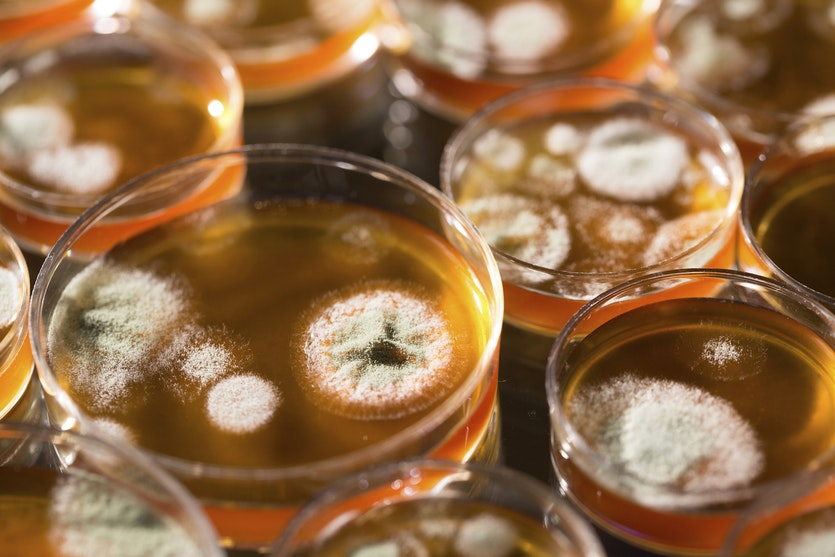
\includegraphics[width=\textwidth,height=1.5625in]{img/190108-dish-full.jpg}

Clustered data:

\begin{itemize}
\item
  Compare two groups (treatment with a control);
\item
  M units (petri plates, persons, animals\ldots) per group;
\item
  Each unit is measured R times. Measurements on same unit are
  positively correlated.
\end{itemize}

\end{block}

\end{frame}

\begin{frame}

Simulated data: Two groups, \(N=3\) subjects per group, \(R=3\)
replicated measurements per subject.

\small

\begin{tabular}{rllrll}
\toprule
y1 & grp & subj & y1 & grp & subj\\
\midrule
67 & ctrl & subj1 & 26 & trt1 & subj4\\
72 & ctrl & subj1 & 45 & trt1 & subj4\\
140 & ctrl & subj1 & 90 & trt1 & subj4\\
13 & ctrl & subj2 & 48 & trt1 & subj5\\
27 & ctrl & subj2 & 53 & trt1 & subj5\\
37 & ctrl & subj2 & 95 & trt1 & subj5\\
-76 & ctrl & subj3 & 70 & trt1 & subj6\\
-66 & ctrl & subj3 & 99 & trt1 & subj6\\
-56 & ctrl & subj3 & 131 & trt1 & subj6\\
\bottomrule
\end{tabular}

\begin{block}{\normalsize}

Problem/issues: If we ignore clustering/positive correlation:

\begin{itemize}
\tightlist
\item
  Pretend to have more information than we have
\item
  Standard errors of estimates become too small
\item
  \(p\) values become too small
\item
  Effects appear stronger than they really are.
\end{itemize}

Notice:

\begin{itemize}
\tightlist
\item
  Measuring the same unit many many times will make the dataset larger,
  but will not really add many more chunks of information (depending on
  the size of the within-subject correlation, of course).
\item
  Instead, more units are needed.
\end{itemize}

\end{block}

\end{frame}

\begin{frame}

\begin{block}{Ignore clustering}

Simple regression model

\[
y_{gir} = \mu + \beta_g + e_{gir}
\]

\small

\begin{table}[!h]
\centering
\begin{tabular}{lrrrrr}
\toprule
  & Estimate & Std. Error & t value & Pr(>|t|) & Pr(>X2)\\
\midrule
(Intercept) & 17.6 & 18.8 & 0.934 & 0.364 & 0.350\\
grptrt1 & 55.4 & 26.6 & 2.086 & 0.053 & 0.037\\
\bottomrule
\end{tabular}
\end{table}

\normalsize

Notice: the \(t\)-test ``accounts for'' the uncertainty in the estimate
of the standard error; gives larger \(p\) values.

\end{block}

\end{frame}

\begin{frame}

\begin{block}{Analyse average}

Compute average for each subject and consider model \[
\bar y_{gi} = \mu + \beta_g + e_{gi}, 
\]

\small

\begin{table}[!h]
\centering
\begin{tabular}{lrrrrr}
\toprule
  & Estimate & Std. Error & t value & Pr(>|t|) & Pr(>X2)\\
\midrule
(Intercept) & 17.6 & 34.0 & 0.516 & 0.633 & 0.606\\
grptrt1 & 55.4 & 48.1 & 1.152 & 0.314 & 0.249\\
\bottomrule
\end{tabular}
\end{table}

\normalsize

Notice: Both tests give large \(p\)-values suggesting no effect at all.

\end{block}

\end{frame}

\begin{frame}

\begin{block}{Model with random effects}

Consider variance component model

\[
y_{gir} = \mu + \beta_g + U_{gi} + e_{gir}
\]

\small

\begin{table}[!h]
\centering
\begin{tabular}{lrrrr}
\toprule
term & estimate & std.error & statistic & Pr(>X2)\\
\midrule
(Intercept) & 17.6 & 34.0 & 0.516 & 0.606\\
grptrt1 & 55.4 & 48.1 & 1.152 & 0.249\\
\bottomrule
\end{tabular}
\end{table}

\normalsize

Notice: \(p\)-values (for \(\chi^2\)-test) same as when analyzing
average. No \(t\)-test available.

\end{block}

\end{frame}

\begin{frame}

\begin{block}{The Kenward--Roger approach}

\begin{itemize}
\item
  Multivariate normal model \[
  Y \sim  N( X \beta, \Sigma)
  \]
\item
  Test of the hypothesis \[
  \Lb (\betab -\bm \beta_0) = 0
  \] where \(\Lb\) is a regular matrix of estimable functions of
  \(\bm \beta\).
\item
  With \(\hat \betab \sim N_d(\betab, \bm\Phi)\), a Wald statistic is \[
  W = [\Lb(\hat\betab - \betab_0)]\transp [L\bm\Phi L\transp]\inv [\Lb(\hat\betab - \betab_0)]
  \] which is asymptotically \(W \sim \chi^2_d\) under the null
  hypothesis.
\end{itemize}

\end{block}

\end{frame}

\begin{frame}

Consider scaled version of \(W\):

\begin{displaymath}
  F = \frac{1}{d} W = \frac{1}{d}(\hat \betab - \betab_0)\transp \Lb\transp [\Lb\transp \bm \Phi(\ssb) \Lb]^{-1}
 \Lb (\hat \betab - \betab_0).
\end{displaymath}

In the computations:

\begin{itemize}
\item
  \(\ssb\) is vector of REML estimates for elements in
  \(\Sigma=\var(Y)\) and
\item
  \(\hat \betab\) is REML estimate for \(\betab\).
\item
  \(\bm \Phi (\sigma) = (\bm X' \bm \Sigma(\sigma) \bm X)^{-1} \approx \cov(\hat \betab)\),
\item
  Asymptotically \(F \sim \frac{1}{d} \chi^2_d\) under the null
  hypothesis
\item
  Think of \(\frac{1}{d} \chi^2_d\) as the limiting distribution of an
  \(F_{d,m}\)--distribution as \(m\rightarrow \infty\)
\end{itemize}

\begin{block}{Kenward and Roger's modification}

To account for the fact that \(\bm\Phi=\var(\hat\beta)\) is estimated
from data, we must come up with a better estimate of the denominator
degrees of freedom \(m\) (better than \(m=\infty\)).

Kenward and Roger (1997)

\begin{itemize}
\item
  replaced \(\bm \Phi\) by an improved small sample approximation
  \(\bm \Phi_A\)
\item
  derived formulas for mean \(E^*\) and variance \(V^*\) of \(F\) (based
  on 1. order Taylor expansion)
\item
  scaled \(F\) by a factor \(\lambda\)
\item
  determined denominator degrees of freedom \(m\) by matching moments of
  \(F/\lambda\) with an \(F_{d,m}\) distribution.
\end{itemize}

\end{block}

\end{frame}

\begin{frame}

Consider variance component model

\[
y_{gir} = \mu + \beta_g + U_{gi} + e_{gir}
\]

\small

\begin{table}[!h]
\centering
\begin{tabular}{lrrrrr}
\toprule
  & statistic & ndf & ddf & F.scaling & p.value\\
\midrule
Ftest & 1.33 & 1 & 4 & 1 & 0.314\\
\bottomrule
\end{tabular}
\end{table}

\normalsize

Notice: Same \(p\)-value as when averages are analysed.

However, analysing averages is not always an option.

\end{frame}

\begin{frame}

\begin{block}{Parametrisk bootstrap}

Consider two competing models: A large model \(f_1(y; \theta)\) and a
simpler sub model \(f_0(y; \theta_0)\).

The test statistic for testing the simpler model under the larger is
\(t_{obs}\).

The \(p\)-value becomes:

\[
 p = \sup_{\theta \in \Theta_0} Pr_{\theta}(T \ge t_{obs}),
\] where supremum is under the hypothesis.

Usually supremum can not be computed. Instead we base \(p\) value on the
parameter estimate: \[
 p^{PB} = Pr_{\hat\theta}(T \ge t_{obs}),
\]

\end{block}

\end{frame}

\begin{frame}

In praxis, \(p^{PB}\) is approximated as:

\begin{enumerate}
\item
  Draw \(B\) parametric bootstrap datasets \(D^1, \dots D^B\) from the
  fitted null model \(f_0(\cdot; \hat \theta_0)\).
\item
  Fit the large and the null model to each of these datasets.
\item
  Compute the likelihood ratio (LR) test statistic for each simulated
  dataset. This gives the reference distribution for the test statistic.
\item
  Compute how extreme the observed test statistic is in the reference
  distribution; this gives the \(p\) value.
\end{enumerate}

\end{frame}

\begin{frame}

Consider variance component model

\[
y_{gir} = \mu + \beta_g + U_{gi} + e_{gir}
\]

\small

\begin{table}[!h]
\centering
\begin{tabular}{lrrr}
\toprule
  & statistic & df & p.value\\
\midrule
LRT & 1.47 & 1 & 0.225\\
PBtest & 1.47 & NA & 0.322\\
\bottomrule
\end{tabular}
\end{table}

\normalsize

Notice: \(p\)-values close to those based on Kenward-Roger
approximation.

\end{frame}

\begin{frame}

\small

\begin{figure}
\centering
\includegraphics{beyond-talk-2020_files/figure-beamer/overlay-1.pdf}
\caption{\(\chi^2\) distribution and simulated reference distribution.}
\end{figure}

\normalsize

\end{frame}

\begin{frame}{Simulation study}
\protect\hypertarget{simulation-study}{}

\small

\begin{tabular}{rllrll}
\toprule
y1 & grp & subj & y1 & grp & subj\\
\midrule
67 & ctrl & subj1 & 26 & trt1 & subj4\\
72 & ctrl & subj1 & 45 & trt1 & subj4\\
140 & ctrl & subj1 & 90 & trt1 & subj4\\
13 & ctrl & subj2 & 48 & trt1 & subj5\\
27 & ctrl & subj2 & 53 & trt1 & subj5\\
37 & ctrl & subj2 & 95 & trt1 & subj5\\
-76 & ctrl & subj3 & 70 & trt1 & subj6\\
-66 & ctrl & subj3 & 99 & trt1 & subj6\\
-56 & ctrl & subj3 & 131 & trt1 & subj6\\
\bottomrule
\end{tabular}

\begin{block}{\normalsize}

\begin{itemize}
\item
  Task: Test the hypothesis that there is no effect of treatment. How
  good are the various tests?
\item
  Simulate data \(1000\) times with divine insight: there is no effect
  of treatment.
\item
  Test the hypothesis e.g.~at level \(5\%\). If test has correct nominal
  level we shall reject about \(50\) times.
\item
  If hypothesis is rejected e.g.~\(100\) times then \(p\) values are
  anti-conservative: Effects appear more significant than the really
  are. That is we draw ``too strong'' conclusions.
\end{itemize}

\end{block}

\end{frame}

\begin{frame}

\small

\begin{table}[!h]
\centering
\begin{tabular}{lrrr}
\toprule
  & 0.01 & 0.05 & 0.10\\
\midrule
lm+F & 0.21 & 0.31 & 0.41\\
lm+X2 & 0.24 & 0.35 & 0.42\\
\underline{avg\_lm+F} & \underline{0.01} & \underline{0.06} & \underline{0.11}\\
avg\_lm+X2 & 0.07 & 0.13 & 0.19\\
mixed+X2 & 0.05 & 0.14 & 0.23\\
\underline{mixed+F} & \underline{0.01} & \underline{0.06} & \underline{0.11}\\
\underline{mixed+PB} & \underline{0.01} & \underline{0.05} & \underline{0.10}\\
\bottomrule
\end{tabular}
\end{table}

\normalsize

\end{frame}

\begin{frame}{Sugar beets - A split--plot experiment}
\protect\hypertarget{sugar-beets---a-splitplot-experiment}{}

\begin{itemize}
\tightlist
\item
  Model how sugar percentage in sugar beets depends on harvest time and
  sowing time.
\item
  Five sowing times (\(s\)) and two harvesting times (\(h\)).
\item
  Experiment was laid out in three blocks (\(b\)).
\end{itemize}

\end{frame}

\begin{frame}[fragile]

Experimental plan for sugar beets experiment

\scriptsize

\begin{Shaded}
\begin{Highlighting}[]
\CommentTok{# Plot allocation:}
\CommentTok{#       |  Block 1       |  Block 2       |  Block 3       |}
\CommentTok{#       +----------------|----------------|----------------+}
\CommentTok{# Plot  | h1 h1 h1 h1 h1 | h2 h2 h2 h2 h2 | h1 h1 h1 h1 h1 | Harvest time}
\CommentTok{# 1-15  | s3 s4 s5 s2 s1 | s3 s2 s4 s5 s1 | s5 s2 s3 s4 s1 | Sowing time}
\CommentTok{#       |----------------|----------------|----------------|}
\CommentTok{# Plot  | h2 h2 h2 h2 h2 | h1 h1 h1 h1 h1 | h2 h2 h2 h2 h2 | Harvest time}
\CommentTok{# 16-30 | s2 s1 s5 s4 s3 | s4 s1 s3 s2 s5 | s1 s4 s3 s2 s5 | Sowing time}
\CommentTok{#       +----------------|----------------|----------------+}
\end{Highlighting}
\end{Shaded}

\normalsize

\end{frame}

\begin{frame}[fragile]

\begin{block}{beets data}

\small

\begin{Shaded}
\begin{Highlighting}[]
\KeywordTok{data}\NormalTok{(beets, }\DataTypeTok{package=}\StringTok{'pbkrtest'}\NormalTok{)}
\KeywordTok{head}\NormalTok{(beets, }\DecValTok{4}\NormalTok{)}
\end{Highlighting}
\end{Shaded}

\begin{verbatim}
##   harvest  block  sow yield sugpct
## 1   harv1 block1 sow3   128   17.1
## 2   harv1 block1 sow4   118   16.9
## 3   harv1 block1 sow5    95   16.6
## 4   harv1 block1 sow2   131   17.0
\end{verbatim}

\normalsize

\begin{itemize}
\item
  A typical model for such an experiment would be: \begin{equation}
      \label{eq:beetsmodel1}
      y_{hbs} = \mu + \alpha_h + \beta_b + \gamma_s + U_{hb} + \epsilon_{hbs},
    \end{equation} where \(U_{hb} \sim N(0,\omega^2)\) and
  \(\epsilon_{hbs}\sim  N(0,\sigma^2)\).
\item
  Notice that \(U_{hb}\) describes the random variation between
  whole--plots (within blocks).
\end{itemize}

\end{block}

\end{frame}

\begin{frame}[fragile]

Using \texttt{lmer()} from lme4 we can test for no effect of sowing and
harvest time as:

\small

\begin{Shaded}
\begin{Highlighting}[]
\NormalTok{beet.lg <-}\StringTok{ }\KeywordTok{lmer}\NormalTok{(sugpct }\OperatorTok{~}\StringTok{ }\NormalTok{block }\OperatorTok{+}\StringTok{ }\NormalTok{sow }\OperatorTok{+}\StringTok{ }\NormalTok{harvest }\OperatorTok{+}
\StringTok{                      }\NormalTok{(}\DecValTok{1} \OperatorTok{|}\StringTok{ }\NormalTok{block}\OperatorTok{:}\NormalTok{harvest), }\DataTypeTok{data=}\NormalTok{beets, }\DataTypeTok{REML=}\OtherTok{FALSE}\NormalTok{)}
\NormalTok{beet.noh <-}\StringTok{ }\KeywordTok{update}\NormalTok{(beet.lg, .}\OperatorTok{~}\NormalTok{. }\OperatorTok{-}\StringTok{ }\NormalTok{harvest)}
\NormalTok{beet.nos  <-}\StringTok{ }\KeywordTok{update}\NormalTok{(beet.lg, .}\OperatorTok{~}\NormalTok{. }\OperatorTok{-}\StringTok{ }\NormalTok{sow) }
\end{Highlighting}
\end{Shaded}

\normalsize

\end{frame}

\begin{frame}[fragile]

Both factors appear highly significant

\footnotesize

\begin{Shaded}
\begin{Highlighting}[]
\KeywordTok{anova}\NormalTok{(beet.lg, beet.noh)  }\OperatorTok\StringTok{ }\NormalTok{as.data.frame }
\end{Highlighting}
\end{Shaded}

\begin{verbatim}
##          Df   AIC   BIC logLik deviance Chisq Chi Df Pr(>Chisq)
## beet.noh  9 -69.1 -56.5   43.5    -87.1    NA     NA         NA
## beet.lg  10 -80.0 -66.0   50.0   -100.0  12.9      1   0.000326
\end{verbatim}

\begin{Shaded}
\begin{Highlighting}[]
\KeywordTok{anova}\NormalTok{(beet.lg, beet.nos)  }\OperatorTok\StringTok{ }\NormalTok{as.data.frame}
\end{Highlighting}
\end{Shaded}

\begin{verbatim}
##          Df   AIC    BIC logLik deviance Chisq Chi Df Pr(>Chisq)
## beet.nos  6  -2.8   5.61    7.4    -14.8    NA     NA         NA
## beet.lg  10 -80.0 -65.99   50.0   -100.0  85.2      4   1.37e-17
\end{verbatim}

\normalsize

However, the LRT based \(p\)--values are anti--conservative: the effect
of harvest appears stronger than it is.

\end{frame}

\begin{frame}[fragile]

\footnotesize

\begin{Shaded}
\begin{Highlighting}[]
\KeywordTok{set.seed}\NormalTok{(}\StringTok{"260618"}\NormalTok{)}
\KeywordTok{KRmodcomp}\NormalTok{(beet.lg, beet.noh)}
\end{Highlighting}
\end{Shaded}

\begin{verbatim}
## F-test with Kenward-Roger approximation; time: 0.07 sec
## large : sugpct ~ block + sow + harvest + (1 | block:harvest)
## small : sugpct ~ block + sow + (1 | block:harvest)
##       stat  ndf  ddf F.scaling p.value
## Ftest 15.2  1.0  2.0         1    0.06
\end{verbatim}

\begin{Shaded}
\begin{Highlighting}[]
\KeywordTok{PBmodcomp}\NormalTok{(beet.lg, beet.noh)}
\end{Highlighting}
\end{Shaded}

\begin{verbatim}
## Bootstrap test; time: 5.68 sec;samples: 1000; extremes: 38;
## large : sugpct ~ block + sow + harvest + (1 | block:harvest)
## small : sugpct ~ block + sow + (1 | block:harvest)
##        stat df p.value
## LRT    12.9  1 0.00033
## PBtest 12.9    0.03896
\end{verbatim}

\normalsize

\end{frame}

\begin{frame}[fragile]

As the design is balanced we may make F--tests for each of the effects
as:

\footnotesize

\begin{Shaded}
\begin{Highlighting}[]
\NormalTok{beets}\OperatorTok{$}\NormalTok{bh <-}\StringTok{ }\KeywordTok{with}\NormalTok{(beets, }\KeywordTok{interaction}\NormalTok{(block, harvest))}
\KeywordTok{summary}\NormalTok{(}\KeywordTok{aov}\NormalTok{(sugpct }\OperatorTok{~}\StringTok{ }\NormalTok{block }\OperatorTok{+}\StringTok{ }\NormalTok{sow }\OperatorTok{+}\StringTok{ }\NormalTok{harvest }\OperatorTok{+}
\StringTok{                }\KeywordTok{Error}\NormalTok{(bh), }\DataTypeTok{data=}\NormalTok{beets))}
\end{Highlighting}
\end{Shaded}

\begin{verbatim}
## 
## Error: bh
##           Df Sum Sq Mean Sq F value Pr(>F)
## block      2 0.0327  0.0163    2.58   0.28
## harvest    1 0.0963  0.0963   15.21   0.06
## Residuals  2 0.0127  0.0063               
## 
## Error: Within
##           Df Sum Sq Mean Sq F value  Pr(>F)
## sow        4   1.01  0.2525     101 5.7e-13
## Residuals 20   0.05  0.0025
\end{verbatim}

\normalsize

\end{frame}

\begin{frame}[fragile]{Final remarks}
\protect\hypertarget{final-remarks}{}

\begin{itemize}
\item
  Satterthwaite approximation of degrees of freedom on its way in
  \texttt{pbkrtest}. Faster to compute than Kenward-Roger scales to
  larger problems.
\item
  \texttt{pbkrtest} available on CRAN
  \url{https://cran.r-project.org/package=pbkrtest}
\item
  devel version on github:
  \texttt{devtools::install\_github(hojsgaard/pbkrtest)}
\end{itemize}

\end{frame}

\begin{frame}[fragile]

\begin{itemize}
\tightlist
\item
  \texttt{pbkrtest} described in Ulrich Halekoh and SH (2014)
  \href{https://www.jstatsoft.org/article/view/v059i09}{A Kenward-Roger
  Approximation and Parametric Bootstrap Methods for Tests in Linear
  Mixed Models The R Package pbkrtest}; Journal of Statistical Software,
  Vol 59. Please cite if you publish results using the package.
\end{itemize}

Thanks for your attention!

\end{frame}

\end{document}
